\section{Reply to comments (only for public defense)}
\begin{itemize}

\item We tackle the issue of the representativeness of publications by university professors and academic scholars in detail in Appendix \ref{appendix:data1}. We look at Italian scientists who gave their name to a crater on the moon. The fact that a large majority of them were either university professor or member of an academy (or both) comforts the idea that our sample of scholars is a good representation of people working in sciences.
\item We tackle the issue of how much of the Italian University/Academy population is covered in detail in Appendix \ref{appendix:data2}. In brief, we think that we have excellent coverage of University Professor, while we probably miss many members of the academy. In appendix \ref{appendix:c} we show that excluding members of the academies does not change the main conclusions of our analysis.
\item Before the public defense, table~\ref{tab:publi} showed only the comparison between Italy and Europe. Both Matthias and Luca pointed out that it would be interesting to see a comparison between Italy and other European countries singularly. This exercise is interesting for many reasons, among which: $i)$ the comparison between Europe and Italy can be driven by one country alone; $ii)$ the overtake might be driven by a change in the composition of European scholars over time; $iii)$ some catholic countries like France or Belgium might be more interesting comparisons to Italy than Europe as a whole. Hence, we updated table~\ref{tab:publi} to contain different European countries taken singularly: before the introduction of the Index in the second half of the $16^{th}$ century knowledge production in Italy is the largest, except for those countries for which we have very few observations. We can also observe that after the introduction of the Index Italy is overtaken by all (except for Spain and Portugal) the European countries we considered. Overall, these data confirm that Italy lost its primacy in knowledge production, being overtaken by several European countries. We did not show the results for all European countries because they had too few observations or contained scholars coming from one University/academy only.

The comparison between Italy and other European countries in table~\ref{tab:publi} also shows that the latter reach a level of knowledge production unknown to Italy. This fact speaks against the possibility that Italy was overtaken because it had less room for growth and that Europe grew more just because of a spreading of knowledge in more remote areas. 

\item The number of published scholars rose steadily in early modern Europe, as pointed out by Matthias. One issue with this is that the observed decline in knowledge production might be due to a weakening of the barriers to entry into the scholar profession. In fact, if published scholars are positively selected and the barriers to entry weaken, the average quality of scholars goes down. One way to control for this problem is to look at the dynamics of top scholars, who are less affected by changes in the barrier to entry. Hence, in table \ref{table:europewiki} in the appendix, we show that Italy loses to Europe in terms of knowledge production also if we consider only scholars whose Wikipedia page is longer than 5000.

	\item One point raised by Luca is that major events in Italian history led to an impoverishment of the peninsula. As a consequence, the production of knowledge slowed down. This is an important point, and it is complementary with other hypotheses of the economic decline of Italy that we briefly presented in the introduction \cite{land99,braudel2018,gusdorf1971}. While this mechanism is reasonable and I believe it had a relevant role, I don't think it is the main force in explaining why North and West Europe overtook Italy in knowledge production. This is because most European countries overtook the GDP per capita of Italy after 1750 (see Figure \ref{fig:gdppc}), while Italy lost its primacy in knowledge production much earlier and in coincidence with the first issues of the Index librorum prohibitorum, as documented by Table~\ref{tab:publi}. 
\begin{figure}[ht]
	\centering
	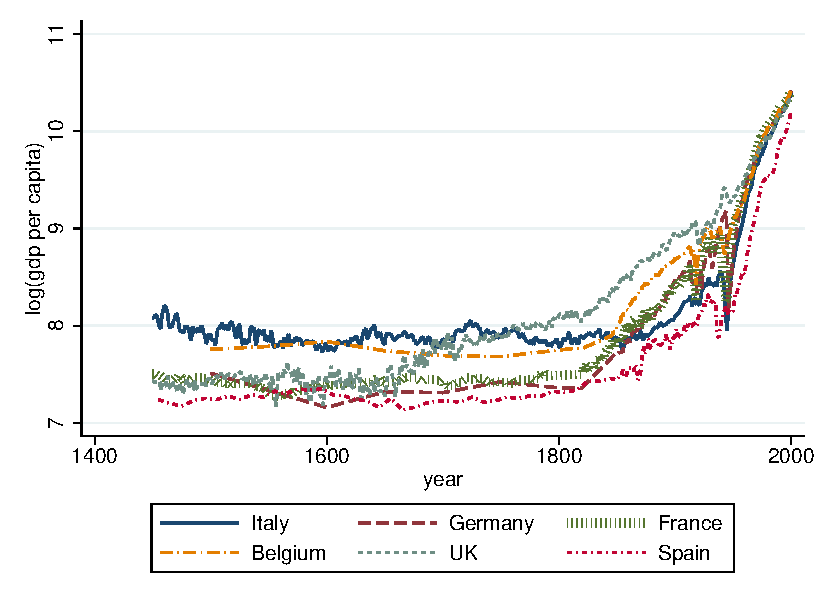
\includegraphics[width=0.7\linewidth]{gdppc.pdf}		
	\caption{Log GDP per capita according to \protect\citeN{bolt2020maddison}.}
	\label{fig:gdppc}
\end{figure}
\FloatBarrier

\item One question by Luca was whether we observe a geographical gradient in censorship. Figure~\ref{fig:italy} shows the place of birth of the scholars in the database, distinguishing the censored (red) from the not censored (green) ones. We retain that our data covers the whole peninsula and its island without obvious bias from Italy's map. Moreover, censorship seems to affect all regions. Another question is whether censorship was actually enforced: we discuss this issue in subsection \ref{subsection:modela}.

\item About differences in censorship in Italy and Europe. Both Italians and non-Italians are present in the Index of forbidden books. We focused on Italy because historians claim that censorship was better enforced there. One explicative example is the story of Copernicus’ \textit{De revolutionibus}, which was first published in 1546 and appeared in the Index in 1616 under the list of books to be corrected. \citeN{gingerich2004} analyzed 277 copies of the first edition and 324 of the second of \textit{De revolutionibus}. He found that about two-thirds of the copies of \textit{De revolutionibus} in Italy were "corrected." \footnote{Since the \textit{De revolutionibus} could circulate for decades without any problem, two-thirds is probably a lower bound estimate of the overall rate of enforcement. One copy forgotten in a private library for decades is probably less likely to be corrected.} However, virtually none of the copies outside Italy, among which Spain and France, were touched. 

\item Europe overtook Italy in terms of scholars quality. In principle, this could be driven by the mere fact that a field with low average publications became relatively more common in Italy than in Europe. To reply to this point, in appendix \ref{appendix:data3} we show the dynamics of scholars quality in Italy and Europe by field. In summary, we observe two features: $i)$ the share of publications in science and medicine rises much faster in Europe than in Italy; $ii)$ concerning scholars quality, Europe overtakes Italy in each field at the time censorship was introduced. This analysis is consistent with the effect of censorship in the model, according to which the Index $i)$ affects the occupational choice of scholars; $ii)$ decreases quality within sectors/fields.

\item In the model, we do not allow for the possibility that there is a limit to growth in the compliant sector. One way to consider this possibility is to assume that books quality in the compliant sector cannot exceed a certain limit. This limit could be equal to the unconstrained average quality in the compliant sector: this choice would capture both the bounded nature of the compliant sector and the fact that the upper limit can shift over time. This is consistent with \citeN{benabou2015}, which shows that religious institutions can adapt the doctrine to the arrival of new knowledge. Allowing for this possibility in our model is perfectly feasible, but it requires some time as all the code that simulates the model needs to be rewritten. I think that the main conclusion of the model would not change much: in fact, the main restriction of the model, namely the link between the relative productivity in the two sectors and the share of revolutionary ideas, would still be in place.

\item As it was pointed out during the defense, one problem with our measure of authors' quality is that it may be biased because older works have more editions. To limit this problem, in appendix \ref{appendix:c} we consider a different measure of author's quality, based on the number of characters of the author's longest Wikipedia page. Table \ref{table:robust} shows that our results are robust to this different measure of quality.

\item Clarification about the domains of revolutionary and compliant knowledge. Being compliant does not necessarily mean to produce using the official Roman Church doctrine as an input: this is true just for the production of religious books or religious services in general. Instead, it just means that the knowledge should not contradict the Roman Church doctrine. This in accordance with data: (new) figure \ref{fig:censdis} documents that we can find censored authors (who necessarily belong to the revolutionary sector) belonging to any field, from Theology to Sciences.

\item Clarification about the distribution and access of knowledge in Italy and Europe. The model is estimated using data from Italian scholars. This does not mean that Italians cannot access knowledge from other scholars in Europe: the database actually includes many non-Italians that were members of an Italian Academy of taught in an Italian University. The sample of foreigners active in Italy is probably not representative of the overall knowledge in Europe, but I think it can give a better picture of the European knowledge that was relevant for Italians. In fact, if a non-Italian scholar did not bear knowledge relevant for italians, she or he would probably no be invited to join an Italian Academy or University.


\item Clarification about $k_1^R, k_1^C$. In the introduction and estimation section we clarified that we do not assume $k_1^R>k_1^C$, which are estimated instead. Interestingly, we did non include the initial quality of censored and non-censored books (which are tightly linked to $k_1^R$ and $k_1^C$) among the target moments, but the model can reproduce them. This means that the data do not reject the one-to-one relationship between the share of revolutionary ideas and relative quality by sector.

\item Question: why do you have that $k_1^R>k_1^C$? Understanding why the initial stock of revolutionary knowledge is larger than that of compliant knowledge in not an easy task, as many factors can in principle contribute to this gap. While this fact deserves further investigation, it is not surprising. In fact, the $15-16^{th}$ centuries was the period of the Renaissance, which favored the blossoming of buoyant ideas.

\item Question: how do you account for the migration of scholars? I agree with Luca when he says that scholar's migration to avoid censorship could be a driver of the decline in knowledge production in Italy. I think we partially capture this in a reduced form way in the model version with self-censorship. One scholar that migrates to publish his heretic ideas can be interpreted in the model like a scholar that self-censor and decides not to publish his heretic book.


\item About the possibility that better books have more readership. This possibility can be embodied in our model by reinterpreting parameter $\mu$. Assume that readers visit a number $B$ of bookshops and buy the best among $\hat{\mu}$ books for each bookshop. Then, readers retain the best book among all the books they bought. This situation is equivalent to our model if $B\hat{\mu}=\mu$ and high-quality books will have relatively more readership.


\item Question: do you allow for the possibility that high-quality work facilitates the creation of new high-quality knowledge? Yes: in our specification, parameter $\nu$ multiplies $b_t^i$.  

\item Clarification about Footnote 12. I agree that rulers have the final say about the religion of their territory, but I also think that their decision is not completely independent from the common people's believes. Protestantism could spread thanks to the invention of the printing press, which aroused popular support by distributing pamphlets \cite{eisenstein1980,rubin2014}. Probably it would not be the best choice for a ruler to impose Catholicism if a large majority of its population already converted to Protestantism.

\item Question about the number of parameters and moments in the estimation. About the estimation, we could have added mode moments in the estimation but this would have brought little identifying information. For example, we used to have the dynamics of quality of censored authors (additional 8 parameters) as target moments but we dropped them once we realized that they did not help to identify the parameters. In fact, when we dropped them, the parameter estimates did not change significantly. The relatively low standard errors of the parameters (see figure \ref{table:param}) suggest that our target moments are sufficient to identify the parameters.

\item Question about the validity of our model before 1400 and clarification about parameter $\psi$. Our model describes the behavior of the Church and scholars from 1400, while I do not think that it is a good description of what happened before. This is because before the invention of the printing press, books were more expensive and hence the spread of heretic ideas through books was less likely. In this context, setting up a censorship apparatus was probably not the priority for the Church. In subsection \ref{subsection:modela} we discuss why we chose to model the cost of censorship as a one-shot fixed cost  $\psi$.
I agree that it would be better if $\psi$ was identified by moments that relate directly to the cost of setting up a censorship apparatus. Since this is unfortunately not feasible, we had to think about a different strategy to set $\psi$. Since in our model the Church postpones the introduction of censorship because of impatience, it seemed natural to identify $\psi$ by the timing of censorship. 
\item In the estimation section, I clarified the sentence related to $p$ ``This assures that the initial[…]'' by providing an example. If $p$ was equal to 1, the share of censored authors would converge to 1 very fast: as a result, the share of censored authors would converge to $\overline{\beta}$ and stay constant, unlike in the data.
\item Clarification: how to interpret parameter $p$. The way it should be interpreted is rather wide, as it summarizes all the reasons why a customer should prefer a compliant rather than a heretic book that has the same quality . I agree that $p$ might have changed over time: this is partially taken into account in the self-censorship version of the model. In fact, equation \ref{eq:censorhip2} shows that the introduction of self-censorship can be interpreted as a change in $p$: $p_{\text{after censorship}}=\gamma p$.



\item Clarification about the use of log(publications). For each scholar, we use the Worldcat search engine to assign to each person all the written output she/he generated, including post mortem editions. More precisely, we count the number of ``publications'' by the person. These include different editions of the same work, and for this reason, top scholars can have thousands of publications. Since the distribution of publications is extremely right-skewed, we proxy the quality of scholars by log(publications.)


 \item Corrected a typo on the definition of $q$, which appeared with two apparently with different meanings.
\end{itemize}

